% Molecular Electronics and Dynamics
\subsubsection{Quantum Dynamics in Molecular Systems}
\index{Kleinekath\"ofer, Ulrich} \label{Nano:Kleinekathoefer}

\paragraph{Research Team}
Ulrich Kleinekath\"ofer (Professor), GuanQi Li (PhD Student), J\"org Liebers
(Diploma Student, still TU Chemnitz), Carsten Olbrich
(PhD Student), Soroosh
Pezeshki (PhD Student), Markus Schr\"oder (PhD Student)\\

%150 words about research in general

Quantum dynamics is one major research focus of our computational physics
group. For the calculation of nonlinear spectra of small molecules such as
the iodine molecule in gas phase wave packet calculations are being
performed to reproduce and interpret spectra obtained in the group of
Prof.\ Materny. When the dynamics takes place within a liquid environment,
dissipation effects have to be added to the quantum dynamics which is
accomplished by the coupling to a thermal bath.  The emerging density
matrix formalism then allows for a simulation of electron and excitation
transfer processes for example in DNA. Similar techniques can be used to
derive quantum master equations for the transfer of electrons trough
molecular wires. The developed formalism allows to treat the laser-matter
interaction accurately. Scenarios are being developed in which ultrafast
laser pulses control the current through the molecular wire.


\paragraph{Highlights}

%500 words about highlights in 2006

\emph{Molecular wires:} The influence of Gaussian laser pulses on the
transport through molecular wires is investigated within a tight-binding
model for electrons with and without spin including electron-electron
interaction. Motivated by the phenomenon of coherent destruction of
tunneling for monochromatic laser fields, situations were studied in which
the maximum amplitude of the electric field fulfills the conditions for the
destructive quantum effect.  It was shown that, as for monochromatic laser
pulses, the average current through the wire can be suppressed.  For
parameters of the model, which do not show a net current without any
optical field, a Gaussian laser pulse can establish a temporary current. In
addition, the effect of electron correlation on the current was
investigated.


\begin{figure}[ht]
  \begin{center}
    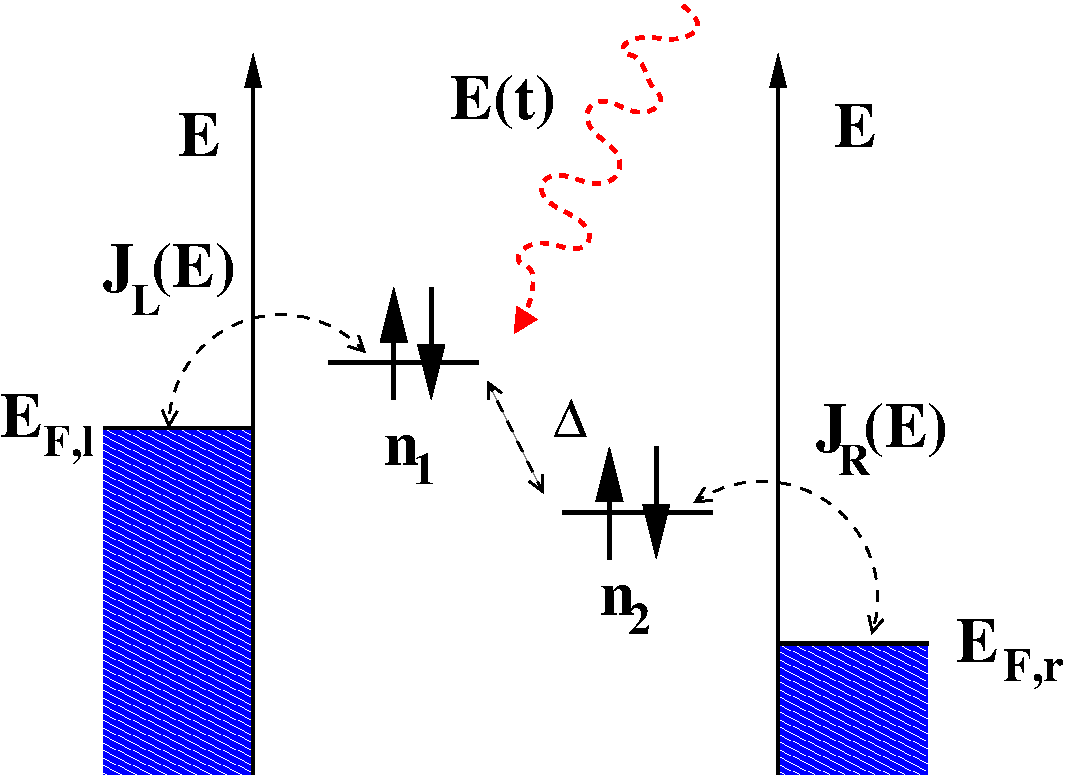
\includegraphics[width=5.5cm]{Kleinekathoefer/kleinekathoefer_fig2.pdf}
    \mycaption{A two-site molecular wire coupled to two electronic
      reservoirs.  The on-site energies $E_n$ of the wire can be
      manipulated with a time-dependent external electric field $E(t)$.}
 \label{fig:profkleinekathoefer2}
   \end{center}
\end{figure}





\emph{Nonlinear spectroscopy and coherent control:}

To shape vibrational wave packets in the iodine molecule we used
perturbation theory and optimal control theory.  The third-order perturbed
wave packets are shaped by using three pulses, i.e.\ two Gaussian pulses
with fixed parameters and a control pulse. In further simulations we
changed the control goal so we were able to modify and control fs-CARS
(coherent Anti-Stokes Raman scattering) spectra. We were able to either
enhance the whole spectrum and its transients or a frequency interval.
Presently these theoretical results are extended by including rotational
effects of the molecules. This  will enable us to make direct
comparisons to experiments being performed in the laboratory of Prof.\
Materny.  Furthermore we are studying the theory of non-resonant fs-CARS
spectra. For this projection operator techniques are being
applied.
 \newline \newline Ulrich Kleinekath\"ofer is also involved in
``Biocomputing".

\paragraph{Collaborations}
\begin{enumerate}
\item {\sl International University Bremen} \\ Prof.\ Arnulf Materny
  \\ Calculation of nonlinear spectra and coherent control
\item {\sl Technische Universit\"at Chemnitz} \\ Prof.\ Michael Schreiber
  \\ Electron transfer in molecular systems
\item {\sl Humboldt Universit\"at zu Berlin}
  \\ Priv.-Doz.\ Dr.\ Volkhard May
\\ Determination of nonresonant spectra and optimal control
\item {\sl Bremen Center for Computational Material Science}
  \\ Prof.\ Thomas Frauenheim \\ Quantum transport in molecular wires
\end{enumerate}


\paragraph{Grants}
\begin{enumerate}
\item Funded by DFG, \emph{light-harvesting complexes}, KL
  1299/3-1 (October 2006 - September 2008)
\item Funded by DFG, priority program SPP 1243 \emph{Quantum transport
  at the molecular scale}, KL 1299/4-1 (November 2006 - December
  2008)
\end{enumerate}

\nocite{profkleinekathoeferwela05a}
\nocite{profkleinekathoeferschr05a}
\nocite{profkleinekathoeferwela05b}
\nocite{profkleinekathoeferklei06a}
\nocite{profkleinekathoeferklei06b}
\nocite{profkleinekathoeferklei06c}


%Publications should be delivered as a separate file (naming
%convention profxxx.bib. See description by R. Helling. Please make
%sure that all your publications are referred to in the TiX file.
%This can either be in form of a \cite{profxxxkey} or as a
%\nocite{profxxxkey} in the end. A publication which is not
%reffered to on the LaTeX file doesn't produce any output in the
%report.
